%!TEX root = main.tex

\section{LIDA}
\label{sec:lida}
LIDA is both the name of a cognitive model and a software framework based on the cognitive model.

\subsection{The LIDA model}
\begin{figure}[h!tb]
\centering
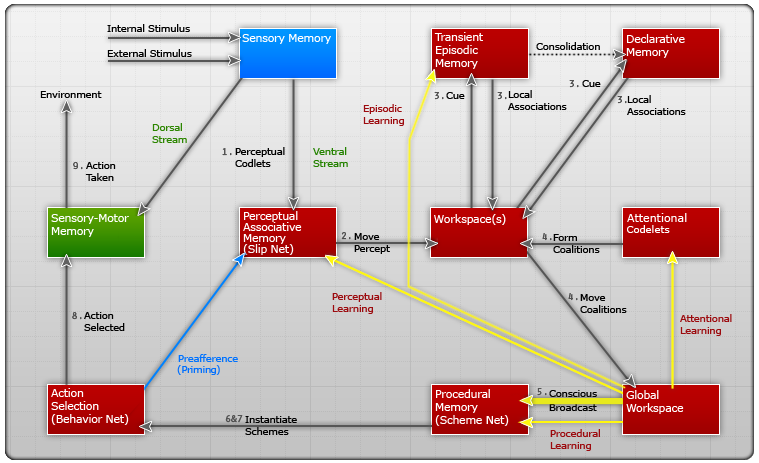
\includegraphics[width=\textwidth]{graphics/lida-model.png}
\caption{Overview of the LIDA cycle.\cite{franklin2007lida}}
\label{fig:lida-cycle}
\end{figure}

The LIDA model is a conceptual and computational model that describes cognition. It is based on the General Workspace Theory, which is a theory to describe functional consciousness. It incorporates and accounts for a large number of psychological and neuropsychological theories.\cite{Franklin2012}

\subsubsection{The LIDA cognitive cycle}
The computational model of LIDA views the artificial agent's ``life'' as a series of cognitive cycles. A high-level, simplified view of how this cognitive cycle is modeled in LIDA can be seen in figure \ref{fig:lida-cycle}. The cognitive cycle itself is subdivided into three separate phases; the understanding phase, the consciousness phase and the action selection phase.

\paragraph{Understanding phase}
In the understanding phase sensory input is tagged with semantic meaning. First low-level feature detectors in the Sensory Memory are run on the incoming stimuli. The output from these is passed onto the Perceptual Associative Memory. There higher-level feature detectors are run, which recognise abstracted entities like objects, events, actions, etc. The output of these is sent to the Workspace, from where it is pushed to both the Transient Episodic Memory and the Declarative Memory. Local associations generated from these memory modules are combined with the percept to generate a Current Situational Model, which is the agent's ``inner map'' of how the world looks.
\paragraph{Attention phase} Parts of the Current Situational Model is composited together to coalitions by Attention Codelets. These coalitions are put into the Global Workspace. From the Global Workspace a codelet selects the coalition in most need of conscious attention and broadcasts this.
\paragraph{Action selection phase} The Action Selection module takes in possible action schemes (behaviours) from the Procedural Memory, and selects one of these according to a competetive process. The selected action scheme is sent to the Sensory-Motor Memory, where it is executed. This method of action selection is based on Maes' behaviour net.\cite{maes1989right} Learning is also done in the action selection phase. In the Perceptual Associative Memory new entities and associations are created and old ones are reinforced during this phase. In the Transient Episodic Memory events from the broadcast from the Global Workspace are stored. The Procedural Memory stores new possible action schemes from the broadcast, and reinforces old ones.


\subsubsection{The workspace}
The workspace is composed of three main modules; the Current Situational Model, Scratchpad and the Conscious Contents Queue.

\paragraph{Current Situational Model} This is where the internal ``map'' of the agent is represented. This contains current events that are linked to associations. Various structure-building codelets running in the Workspace are responsible for building these.
\paragraph{Scratchpad} The Scratchpad is used for temporary storage for the codelets while they build up structures before moving into Current Situational Model.
\paragraph{Conscious Contents Queue} This contains a list of previous broadcasts, which allows LIDA to take time into account, and reason on things that happens over time.

\subsection{LIDA framework}
\subsubsection{Background}
The LIDA framework implements a growing subset of the full computational LIDA model in a re-usable Java-based software framework.

While LIDA seems to have started simply as an extension for the IDA agent with added learning modes,\cite{franklin2007lida} it has evolved into a generic AGI framework, which can be used for other models than LIDA, because of the modular nature of the framework.\cite{snaider2011lida}

The reason for using a framework is that software projects implementing cognitive models tend to grow fairly large and complex therefore difficult to both implement in the first place and maintain over time.

Various types of frameworks, like the Qt application framework or Ruby on Rails web application framework, have been successfully used in software development for a long time to simplify and ease the implementation software projects\cite{bachle2007rails}.

They do this by providing pre-built functionality, a shared platform that can be improved and worked on by everyone who uses it, and also promotes collaboration between users of the framework. And since the amount of custom code that has to be maintained in the individual projects decrease significantly the burden of maintainence eases as well.\cite{snaider2012lida}

\subsubsection{Features}
The LIDA software framework contains default implementations of the major modules in the LIDA model as well as abstract classes for the generic parts of the model, which needs to be implemented in an agent.

The main parts of it are the modules, tasks, common internal representations, a task manager, a GUI, an object factory, strategies and also an XML parser for the agent description files.\cite{snaider2012lida}

\subsubsection{Modules}
The modules are collections of tightly coupled data and processes that operate on them. The coupling between the various modules usually is very loose, however.

Domain independent modules in the LIDA model have full implementations in the framework, while domain-dependent ones only have abstract implementations that has to be provided by implementations that use the framework.

Modules are arranged in a hierarchy; for example the Workspace module has a submodule that represents the Current Situational Model. 

Communication between modules is done with the Observer design pattern, where objects registers interest in other objects by calling their {\em addListener} methods, and then get callbacks to pre-defined methods whenever there are updates. An example of this is the GlobalWorkspace-class, which implementations of BroadcastListener can listen to.

The modules with default implementations in the current version of the LIDA framework are as follows:\cite{snaider2012lida}
\begin{itemize}
 \item Environment (abstract)
 \item Sensory Memory (abstract)
 \item Perceptual Associative Memory
 \item Transient Episodic Memory
 \item Declarative Memory
 \item Workspace
 \item Structure-Building Codelets
 \item Attention Codelets
 \item Global Workspace
 \item Procedural Memory
 \item Action Selection
 \item Sensory-Motor Memory
\end{itemize}

\paragraph{Environment} This is an abstract class, since it is highly domain-dependent, and it has to be provided by the user of the framework. The implementations need to implement at least getState and processAction.
\paragraph{Sensory Memory} This is also highly domain-dependent, and therefore has no default implementation.
\paragraph{Perceptual Associative Memory} Here all the nodes available from the environment are, together with their current activation level.
\paragraph{Transient Episodic Memory} This is the short-term episodic memory. This module stores events from the conscious broadcast for a short term, with a quick decay.
\paragraph{Declarative Memory} This is the long-term episodic memory, with a slow decay. Entries in the Transient Episodic Memory are moved here if they haven't decayed for a long period of time.

Both the declarative and transient episodic memory are implemented as sparse distributed memory.\cite{kanerva1988sparse}
\paragraph{Procedural Memory} This module contains behaviour schemes that are used to instantiate behaviours. Instantiated behaviours from this are sent to the action selection from procedural memory.
\paragraph{Action Selection} In the current version of the framework this is implemented as a simple rule-based system, however in version 1.2 this is replaced with a behavioural net, inspired by Maes' nets.\cite{maes1989right}

\subsubsection{Tasks}
These are small processes implemented as short-lived algorithms that reflect the {\em codelets} and other processes in the LIDA model. The implementation class is called {\em FrameworkTask}.

Tasks are spawned by a separate class, the TaskSpawner, which classes that need to spawn tasks interact with. Tasks are scheduled for execution at particular ``ticks'', which are the time units used in the framework. The task manager runs the Task's ``runThisFrameworkTask'' method each time it is scheduled for execution. Tasks can either be run once, or repeatedly, depending on the type of task it is. For example an ExciteTask, which is used for passing activation, is run once, while feature detector tasks are run repeatedly on input.

When a task has finished executing it is returned to the TaskSpawner which processes the results and decides whether the task should be rescheduled for execution.

\subsubsection{Common internal representations}
To make modules able to efficiently collaborate on information and data, there are several common internal representations used for data in the framework.

{\em Nodes} and {\em Links} are the two major data structures used for representing information in the LIDA framework.

Nodes are data structures that can represent anything needed in an agent, both concretely or more abstract, like features, objects, events, concepts, feelings, actions, etc. Every Node has a reference to a PamNode from the Perceptual Associative Memory, from which it originates, as well as a unique ID.

Links represents connections between Nodes. The framework differentiates between simple links, which links between two Nodes, and complex links, which links to other links. Links have a LinkCategory that describes the nature of the Link; for example a Link connecting two Nodes ``ball'' and ``red'' might have the category ``feature'', for a representation of a red ball. 

Both Links and Nodes implement the {\em Linkable} interface, and contains a unique ID represented by a variable named {\em ExtendedId}.

It is also possible to have custom subclasses of both Link and Node with custom properties and functionality.

All instances of Link and Node, both default and custom subclasses, are created by the element factory.

The common internal representation used for sending information between modules is usually a NodeStructure, a graph structure composed of Nodes and Links. The default NodeStructureImpl has a default implementation of methods for managing the elements in it (adding, removing, retrieving, merging, etc.). An important point to note is that when an element is added, a copy is made and added instead, because adding the same Java object to several node structures could have significant, unforeseen circumstances (where operating on data in one structure affects a completely unrelated one).

\subsubsection{Task manager}
The task manager is responsible for the dispatching (when called from the TaskSpawner) and execution of the tasks, usually parallelized. This is similar to the CRANIUM software in the CERA-CRANIUM architecture described in Section \ref{sec:cogarch}. It is also responsible for keeping track of the internal time representation, the ``ticks''.

Tasks are organized in a queue, sorted according to the tick they are scheduled for. The task manager main loop consists of four steps; First it decays the activation level of all the modules, then it executes all the tasks scheduled for the current tick, thirdly it updates the GUI and then increments the tick. This loop is controlled by the public start/pause methods, which are also exposed in the toolbars in the GUI.

The task manager also has a {\em tick duration}, which is the minimum amount of time a tick takes. This can be used to be able to slow down execution if one wants to inspect what goes on. This only is used if the minimum tick duration is longer than the actual time used by the tasks. If the thread pool available to the task manager is larger than one, then several tasks might run in parallel, but still in one tick. Both the tick duration and the thread pool size is set in the configuration file, and the tick duration can also be controlled interactively from within the GUI.

\subsubsection{Activation}
The {\em activation level} describes the {\em salience} (their relative value) of the various elements in the framework that implements the Activatible interface. This includes the nodes, links, coalitions, codelets, schemes, behaviours and more.

The activation level is represented by a decimal value between $0.0$ and $1.0$. The Activatible interface has two methods for controlling the activation level; {\em excite} and {\em decay}, and elements are usually removed if their activation level drops beneath a certain threshold (referred to as a {\em removal threshold} in the framework). These are controlled by separate elements, Strategies (described below), that are easily replacable and interchangeable.

Learning is also done as an extension to the Activation interface, by providing a {\em base-level activation}, which can for example represent the usefulness of a node in the past. We won't go into detail about the Learnable interface here, as the current version of the LIDA framework doesn't ship with any learning algorithms that use this interface.

\subsubsection{GUI}
The framework contains a highly customizable GUI that can be used to inspect every aspect of the implemented model at runtime, as well as provides a way to control the execution.

The appearance of the GUI is controlled by a ``GUI Panels'' property file which describes which custom and default panels are to be displayed in the GUI.

\subsubsection{Strategies}
Strategies encapsulate various algorithms that are shared between modules. Examples of Strategies are the decay and excitation strategies for the activation level; sigmoid and linear excitation and decay are the ones that are provided by default.

\subsubsection{XML parser}
Since the agent description is done in an XML file, the framework provides a complete XML parser that loads and creates an in-memory representation of the agent.

\subsubsection{Factory}
This object factory provides a way to easily generate objects for common data structures and strategies. It is highly recommended that elements aren't created directly, but requested from the ElementFactory. This allows for easy addition of new subclasses of for example Node and Link or strategies. It also allows to easily define activation levels, strategies and parameters to be set in the created objects. An example given in the documentation\cite{snaider2012lida} is that of several Nodes with the same NodeImpl class, but with varying excite and decay strategies, and different initial activations.

The element type definitions are defined in the factory data  XML file which is parsed with the included XML parser, and each contains the name which is used when requesting a new object instance from the factory, the class and parameter values.

\subsubsection{Framework initialization}
The classes that does the initialization of the agent are in the {\em initialization} Java package. The main class for starting the initialization is called {\em AgentStarter}, and contains a main method to take in the location of the main configuration file.

\begin{enumerate}
 \item First the main configuration file is loaded, which contains (among other things) the names of the other configuration files.
 \item From there it gets the name of the factory data file, which contains the definitions for the element factory.
 \item Then an instance of the Agent class is created based on the contents of the agent declaration file.
 \item Then the GUI properties file is loaded and all the GUI objects (including custom panels) are created.
 \item Finally the agent and GUI is loaded and displayed.
\end{enumerate}

\subsubsection{Parameter tweaking}
Like any other (partially\footnote{LIDA is generally viewed as hybrid symbolic/sub-symbolic architecture.\cite{duch2008cognitive}}) sub-symbolic artificial intelligence system, parameter tweaking is very important and small changes in the parameters can completely change how the agent behaves and acts. In LIDA there are a lot of activation values and thresholds for when something is counted as activated. 

The feature detectors are the first instances where activation is important. When they discover something from the input they send activation to one or more nodes in PAM, and this activation level will decide how important the model thinks this piece of information is. In addition to this, it will also have cascading effects on the system further down the line. When attention codelets compete about access to the global workspace and consciousness broadcast the activation of the nodes contained in the codelets context together with the initial activation value of the codelet itself makes up the total activation of the codelet. So if some of the nodes have low activation from the feature detectors the codelet that contains that node will also be judged as unimportant. 

Learning base level activations are part of the LIDA model but are not yet implemented in the current version of the framework, so we haven't been able to utilize it. What it implies is that when some nodes have been important in the past this will make them more likely to be important in the future, and this should have an impact on the performance of the agent. 

Both feature detectors and codelets in the framework are implemented as processes that run at specified intervals, defined by the number of ticks between each time they are run. Changing how often a process is run will also impact the agent in not always predictable ways. If you do not detect the presence of some piece of information in time, you might decide on an action that is not the optimal way to handle the situation, which you might have done if you had all the information available to you. If the period between the execution of a feature detector is to long, you can end up with the related PAM node decaying below the threshold for activation between each time the detector is run, but if the detector was run at more regular intervals it would stay activated constantly because the node would receive excitation after each run of the detector. 

All the elements in the LIDA framework that has activation have different parameters for how this activation is received and decayed. Decay of elements are configured differently for different modules. In Declarative Memory elements decay at a very slow rate, if at all, while in PAM they decay during a very short period of time, usually just a few ticks long. The same options for configuration of excitation exists in the framework.

To facilitate easy tweaking of parameters in LIDA most of them can and should be configurable from the XML definition of the agent. This makes changing and testing new values a lot easier then having to rewrite lines of code between runs.
